\section{Introduction}

The computer vision field has converged on a general method for object detection, and a standard evaluation of results.
Efficiency is not a concern of the evaluation metrics, and the methods are not evaluated in an inherently multi-class setting.
However, in most real-world applications of object recognition, performance is time-sensitive and inherently tied to the many-class nature of the world.

In robotics, a small finite amount of processing power per unit time is all that is available for robust object detection if the robot is to usefully interact with humans.
In large-scale detection system deployments, such as for image search, results need to be obtained quickly per image as the number of images to process is large and growing.

In these cases, an acceptable answer at a reasonable time may be more valuable than the best answer given too late.
Furthermore, the value of the answer depends on the target application.

\begin{figure}[ht!]
\center{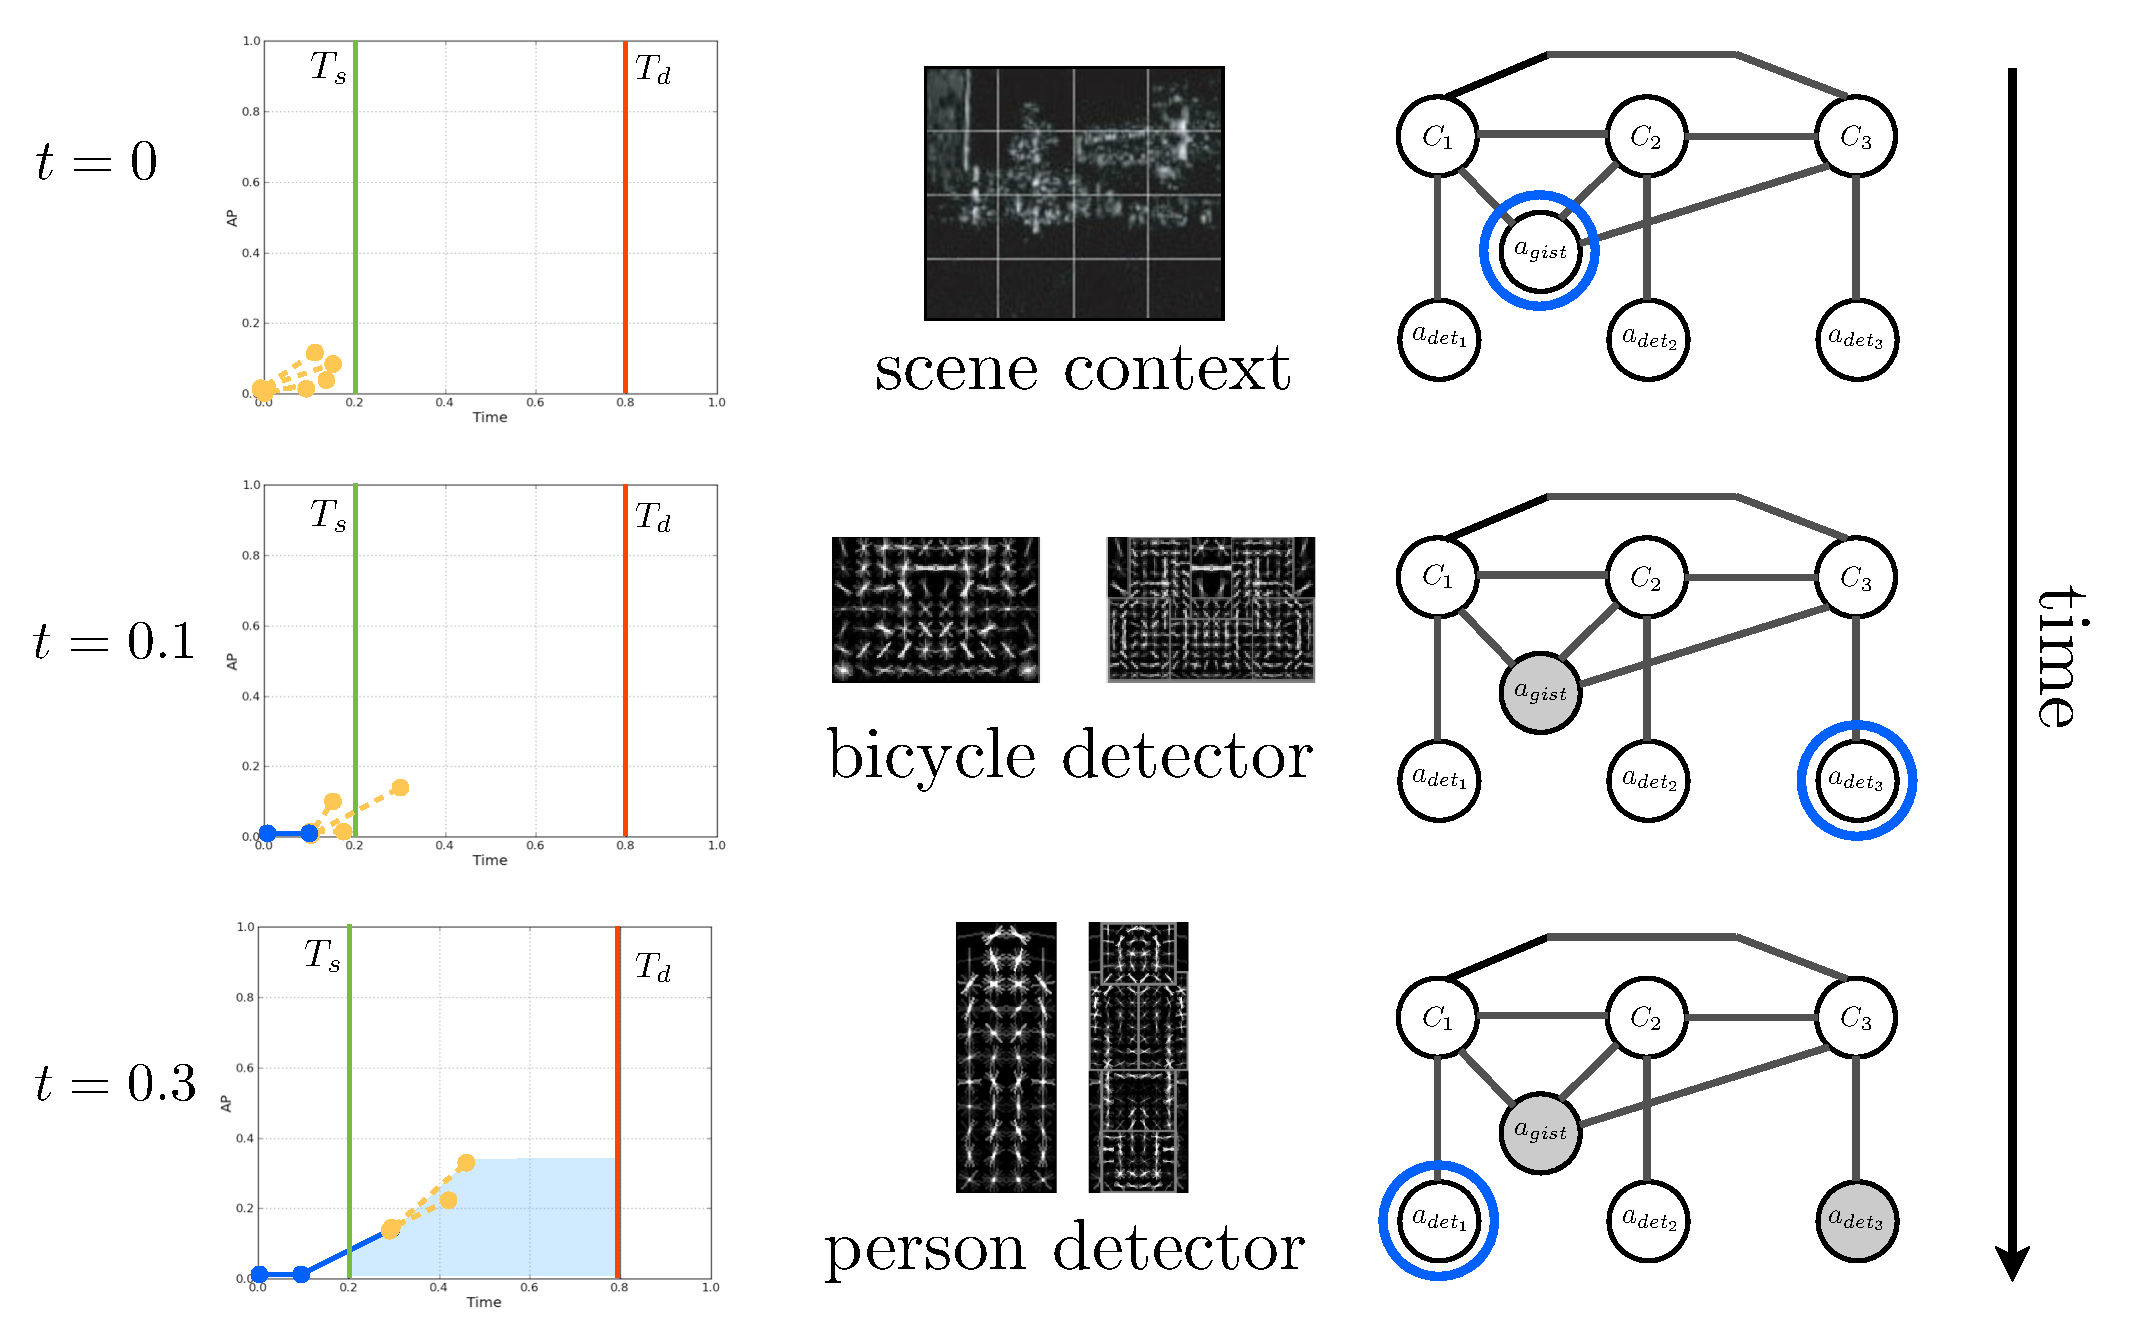
\includegraphics[width=0.86\linewidth]
    {../figures/figure1.pdf}}
  \caption{
A sample trace of our method.
At each time step beginning at $t=0$, potential actions are considered according to their \emph{value}, and the one with the highest value is picked.
The selected action is performed and returns observations, which influence the selection of the next action.
The final evaluation of a detection episode is the area of the AP vs. Time curve between the start and end times.
The value of an action is the expected value of the final evaluation if the action is taken and the policy continues to be followed, which allows actions without an immediate benefit to be scheduled.
}
  \label{fig:figure1}
\end{figure}

A hypothetical recognition system for a vision-based advertising deployment presents a case study.
The system will have different accuracies for objects of different classes; detections will have different values based on confidence and class; and the queue of unprocessed images will vary in size.
The detection strategy to maximize profit in such an environment should depend on all of these variables.

We argue that the key to tackling such problems of dynamic recognition resource allocation is to start asking a new question:
\emph{What is the best performance we can get on a budget?}
To answer it, we consider the evaluation metric of performance vs. time, shown in Figure~\ref{fig:figure1} and discussed further in the text.

We present a method that takes various detectors and classifiers as black boxes, and learns a dynamic policy for selecting detector and other actions to achieve the highest performance under this evaluation.
We are able to obtain better performance than baselines when there is less time available than is needed to run all detectors.
